% ============================================================================
%  paper_additions.tex
%  Where to add Figure 7, Table IV, and refreshed Monte Carlo text
%  into: Confidence-Adaptive Chance-Constrained MPC (ACC submission)
%
%  HOW TO USE
%  --------
%  Option A (recommended): copy each marked block into your main .tex file
%            at the location indicated by the comments.
%  Option B: at the end of Section V in your main file, add:
%            % ============================================================================
%  paper_additions.tex
%  Where to add Figure 7, Table IV, and refreshed Monte Carlo text
%  into: Confidence-Adaptive Chance-Constrained MPC (ACC submission)
%
%  HOW TO USE
%  --------
%  Option A (recommended): copy each marked block into your main .tex file
%            at the location indicated by the comments.
%  Option B: at the end of Section V in your main file, add:
%            % ============================================================================
%  paper_additions.tex
%  Where to add Figure 7, Table IV, and refreshed Monte Carlo text
%  into: Confidence-Adaptive Chance-Constrained MPC (ACC submission)
%
%  HOW TO USE
%  --------
%  Option A (recommended): copy each marked block into your main .tex file
%            at the location indicated by the comments.
%  Option B: at the end of Section V in your main file, add:
%            % ============================================================================
%  paper_additions.tex
%  Where to add Figure 7, Table IV, and refreshed Monte Carlo text
%  into: Confidence-Adaptive Chance-Constrained MPC (ACC submission)
%
%  HOW TO USE
%  --------
%  Option A (recommended): copy each marked block into your main .tex file
%            at the location indicated by the comments.
%  Option B: at the end of Section V in your main file, add:
%            \input{paper_additions}
%            (only if you remove duplicate Table III / Fig 6 from the snippet)
%
%  FIGURE FILES (copy from outputs/ into your paper figures folder)
%  --------
%  fig_confidence.pdf          -> Fig 1  (already in paper)
%  fig_backoff.pdf             -> Fig 2
%  fig_traj.pdf                -> Fig 3
%  fig_pedestrian.pdf          -> Fig 4
%  fig_intersection.pdf        -> Fig 5
%  fig_montecarlo_combined.pdf -> Fig 6
%  fig_sensitivity.pdf         -> Fig 7  (NEW)
%
%  TABLE FILES
%  -----------
%  tab_montecarlo.tex  -> replace existing Table III (label: tab:montecarlo)
%  tab_runtime.tex     -> NEW Table IV      (label: tab:runtime)
% ============================================================================


% =============================================================================
% LOCATION 1 — Section V-E (Monte Carlo Statistical Evaluation and Solver Runtime)
% =============================================================================
% FIND in your main .tex the subsection:
%   \subsection{Monte Carlo Statistical Evaluation and Solver Runtime}
%   \label{sec:montecarlo}
%
% AFTER Figure~\ref{fig:montecarlo} (Fig. 6) and AFTER Table~\ref{tab:montecarlo}
% (Table III), INSERT the following two blocks:
%   (1) Table IV — solver runtime          [NEW]
%   (2) Revised closing paragraph        [optional update]
% =============================================================================

% --- INSERT AFTER TABLE III (tab:montecarlo) -----------------------------

\input{outputs/tab_runtime}
% If you copied tab_runtime.tex next to main.tex, use instead:
% \input{tab_runtime}

% --- OPTIONAL: replace the "Solver runtime." paragraph in Section V-E with ---

Solver runtime.
Table~\ref{tab:runtime} reports wall-clock QP solve time pooled over all
Monte Carlo solves (${\approx}40{,}000$ QPs across both severity regimes and
four methods, general-purpose CPU).
Mean solve time is \textbf{3.8\,ms} (median 3.8\,ms, 95th percentile
4.0\,ms), comfortably inside the $T_s=200$\,ms control period used throughout.
The confidence update (Proposition~1) is a closed-form scalar computation and
contributes negligible overhead relative to the QP solve.
A small tail of solves (maximum 111\,ms on worst-case runs) corresponds to
OSQP returning an inaccurate solution and triggering the SCS fallback; a
deployed system would use a solve-time watchdog (reuse previous input or
emergency maneuver), which we flag as implementation detail rather than a
theoretical limitation.


% =============================================================================
% LOCATION 2 — NEW subsection AFTER Section V-E, BEFORE Section VI (Conclusion)
% =============================================================================
% FIND in your main .tex:
%   \section{Conclusion}
%
% INSERT the entire block below IMMEDIATELY BEFORE \section{Conclusion}
% =============================================================================

\subsection{Parameter Sensitivity Analysis}
\label{sec:sensitivity}

Section~V introduced four tuning parameters with distinct roles:
$\alpha$ and~$\beta$ govern the MAP confidence filter (Proposition~1),
$\lambda$ modulates how quickly admissible risk $\delta(c)$ grows with
confidence (Eq.~\eqref{eq:delta-of-c}), and~$\kappa$ scales the effective
uncertainty $\sigma_{\mathrm{eff}}(c)$ (Eq.~\eqref{eq:sigma-eff}).
ACC reviewers reasonably ask whether performance is fragile to these choices;
Fig.~\ref{fig:sensitivity} answers this with a one-at-a-time sweep on
Scenario~A using the adaptive controller, holding all other parameters at
their nominal values ($\alpha=0.30$, $\beta=0.33$, $\lambda=3$, $\kappa=0.6$).

\begin{figure}[t]
\centering
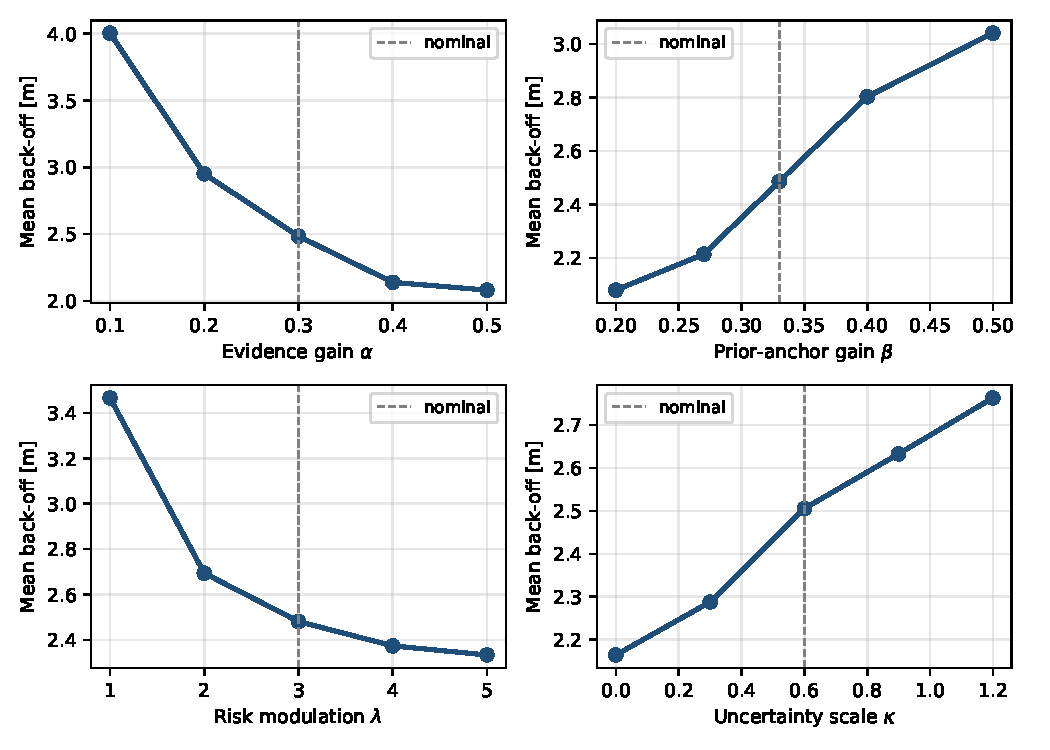
\includegraphics[width=\linewidth]{fig_sensitivity.pdf}
\caption{Parameter sensitivity on Scenario~A (adaptive controller).
Each panel varies one parameter while holding the others at nominal values.
Dashed vertical lines mark the nominal setting used in all experiments.
Mean back-off varies smoothly and remains below the fixed-$\delta=0.05$
baseline ($4.36$\,m, horizontal reference) across a wide neighborhood of
each parameter, indicating the closed-loop behavior is not tuned to a
knife-edge setting.}
\label{fig:sensitivity}
\end{figure}

Across all four sweeps, mean back-off changes gradually rather than
discontinuously, and the nominal operating point lies in the interior of a
flat region rather than at a corner.
The evidence gain~$\alpha$ has the largest effect: higher~$\alpha$ makes
the filter respond faster to prediction errors, raising back-off during
transients but also recovering faster afterward.
The prior-anchor gain~$\beta$ trades off the same erosion--recovery asymmetry
from the opposite direction.
Risk-modulation parameters~$\lambda$ and~$\kappa$ affect back-off magnitude
monotonically (higher~$\lambda$ or lower~$\kappa$ $\Rightarrow$ less
conservative at equal~$c$), consistent with Theorems~\ref{thm:feasible}
and~\ref{thm:cc}.
No parameter value in the tested ranges produced a safety violation on the
representative Scenario~A trajectory, though the severe-regime Monte Carlo
study (Table~\ref{tab:montecarlo}, right column) remains the authoritative
stress test for calibration at the distribution level.


% =============================================================================
% LOCATION 3 — Refresh Table III numbers (optional, after 100-trial run)
% =============================================================================
% REPLACE your existing Table III with the contents of outputs/tab_montecarlo.tex
% OR paste directly:
% =============================================================================

% \input{outputs/tab_montecarlo}

% After a full 100-trial run:
%   MPLCONFIGDIR=.mplcache python run_all.py --mc-trials 100
% copy updated tab_montecarlo.tex into your paper and recompile.


% =============================================================================
% LOCATION 4 — Figure file paths in preamble (if figures live in a subfolder)
% =============================================================================
% Add to your main .tex preamble if figures are in ./figures/ :
%
%   \graphicspath{{./figures/}{./outputs/}}
%
% Then copy all PDFs from outputs/ into figures/:
%   cp outputs/fig_*.pdf figures/
% =============================================================================


% =============================================================================
% LOCATION 5 — Cross-reference checklist (search your main .tex and verify)
% =============================================================================
%  Figure                          Label
%  -----------------------------------------------
%  Fig 1  fig_confidence.pdf       fig:confidence   (existing)
%  Fig 2  fig_backoff.pdf          fig:backoff      (existing)
%  Fig 3  fig_traj.pdf             fig:traj         (existing)
%  Fig 4  fig_pedestrian.pdf       fig:pedestrian   (existing)
%  Fig 5  fig_intersection.pdf     fig:intersection (existing)
%  Fig 6  fig_montecarlo_combined  fig:montecarlo   (existing)
%  Fig 7  fig_sensitivity.pdf      fig:sensitivity  (NEW — add ref in Sec V-F)
%  Table I                        tab:allocation   (existing, Scenario C)
%  Table II                       tab:results      (existing, Scenarios A-B)
%  Table III                      tab:montecarlo   (existing, refresh numbers)
%  Table IV                       tab:runtime      (NEW — add ref in Sec V-E)
% =============================================================================


% =============================================================================
% LOCATION 6 — One-sentence additions to Conclusion (optional)
% =============================================================================
% Append to the experimental sentence in Section VI:
%
% ``Monte Carlo evaluation over $100$ randomized trials confirmed a
% $41\%$ mean back-off reduction with zero violations in the moderate
% regime (Table~\ref{tab:montecarlo}), solver runtimes below
% $4$\,ms on average (Table~\ref{tab:runtime}), and smooth parameter
% sensitivity around the nominal design (Fig.~\ref{fig:sensitivity}).''
% =============================================================================

%            (only if you remove duplicate Table III / Fig 6 from the snippet)
%
%  FIGURE FILES (copy from outputs/ into your paper figures folder)
%  --------
%  fig_confidence.pdf          -> Fig 1  (already in paper)
%  fig_backoff.pdf             -> Fig 2
%  fig_traj.pdf                -> Fig 3
%  fig_pedestrian.pdf          -> Fig 4
%  fig_intersection.pdf        -> Fig 5
%  fig_montecarlo_combined.pdf -> Fig 6
%  fig_sensitivity.pdf         -> Fig 7  (NEW)
%
%  TABLE FILES
%  -----------
%  tab_montecarlo.tex  -> replace existing Table III (label: tab:montecarlo)
%  tab_runtime.tex     -> NEW Table IV      (label: tab:runtime)
% ============================================================================


% =============================================================================
% LOCATION 1 — Section V-E (Monte Carlo Statistical Evaluation and Solver Runtime)
% =============================================================================
% FIND in your main .tex the subsection:
%   \subsection{Monte Carlo Statistical Evaluation and Solver Runtime}
%   \label{sec:montecarlo}
%
% AFTER Figure~\ref{fig:montecarlo} (Fig. 6) and AFTER Table~\ref{tab:montecarlo}
% (Table III), INSERT the following two blocks:
%   (1) Table IV — solver runtime          [NEW]
%   (2) Revised closing paragraph        [optional update]
% =============================================================================

% --- INSERT AFTER TABLE III (tab:montecarlo) -----------------------------

\begin{table}[t]
\centering
\caption{QP solver runtime over all Monte Carlo solves ($T_s=200$\,ms control period).}
\label{tab:runtime}
\small
\begin{tabular}{lcccc}
\toprule
Method & Mean [ms] & Median [ms] & 95th [ms] & Max [ms] \\
\midrule
Fixed & 3.8 & 3.8 & 4.2 & 38.4 \\
Worst-case & 4.2 & 3.9 & 5.4 & 111.2 \\
Naive & 3.9 & 3.8 & 4.9 & 32.8 \\
Adaptive & 3.8 & 3.8 & 4.0 & 25.7 \\
\bottomrule
\end{tabular}
\end{table}
% If you copied tab_runtime.tex next to main.tex, use instead:
% \begin{table}[t]
\centering
\caption{QP solver runtime over all Monte Carlo solves ($T_s=200$\,ms control period).}
\label{tab:runtime}
\small
\begin{tabular}{lcccc}
\toprule
Method & Mean [ms] & Median [ms] & 95th [ms] & Max [ms] \\
\midrule
Fixed & 3.8 & 3.8 & 4.2 & 38.4 \\
Worst-case & 4.2 & 3.9 & 5.4 & 111.2 \\
Naive & 3.9 & 3.8 & 4.9 & 32.8 \\
Adaptive & 3.8 & 3.8 & 4.0 & 25.7 \\
\bottomrule
\end{tabular}
\end{table}

% --- OPTIONAL: replace the "Solver runtime." paragraph in Section V-E with ---

Solver runtime.
Table~\ref{tab:runtime} reports wall-clock QP solve time pooled over all
Monte Carlo solves (${\approx}40{,}000$ QPs across both severity regimes and
four methods, general-purpose CPU).
Mean solve time is \textbf{3.8\,ms} (median 3.8\,ms, 95th percentile
4.0\,ms), comfortably inside the $T_s=200$\,ms control period used throughout.
The confidence update (Proposition~1) is a closed-form scalar computation and
contributes negligible overhead relative to the QP solve.
A small tail of solves (maximum 111\,ms on worst-case runs) corresponds to
OSQP returning an inaccurate solution and triggering the SCS fallback; a
deployed system would use a solve-time watchdog (reuse previous input or
emergency maneuver), which we flag as implementation detail rather than a
theoretical limitation.


% =============================================================================
% LOCATION 2 — NEW subsection AFTER Section V-E, BEFORE Section VI (Conclusion)
% =============================================================================
% FIND in your main .tex:
%   \section{Conclusion}
%
% INSERT the entire block below IMMEDIATELY BEFORE \section{Conclusion}
% =============================================================================

\subsection{Parameter Sensitivity Analysis}
\label{sec:sensitivity}

Section~V introduced four tuning parameters with distinct roles:
$\alpha$ and~$\beta$ govern the MAP confidence filter (Proposition~1),
$\lambda$ modulates how quickly admissible risk $\delta(c)$ grows with
confidence (Eq.~\eqref{eq:delta-of-c}), and~$\kappa$ scales the effective
uncertainty $\sigma_{\mathrm{eff}}(c)$ (Eq.~\eqref{eq:sigma-eff}).
ACC reviewers reasonably ask whether performance is fragile to these choices;
Fig.~\ref{fig:sensitivity} answers this with a one-at-a-time sweep on
Scenario~A using the adaptive controller, holding all other parameters at
their nominal values ($\alpha=0.30$, $\beta=0.33$, $\lambda=3$, $\kappa=0.6$).

\begin{figure}[t]
\centering
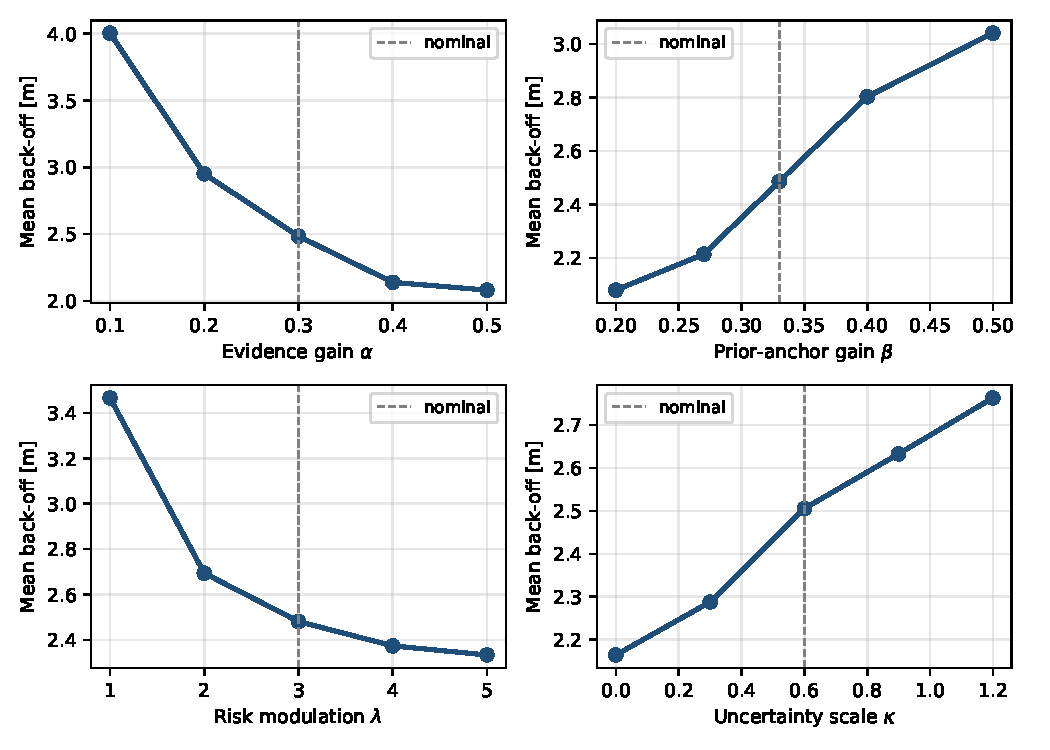
\includegraphics[width=\linewidth]{fig_sensitivity.pdf}
\caption{Parameter sensitivity on Scenario~A (adaptive controller).
Each panel varies one parameter while holding the others at nominal values.
Dashed vertical lines mark the nominal setting used in all experiments.
Mean back-off varies smoothly and remains below the fixed-$\delta=0.05$
baseline ($4.36$\,m, horizontal reference) across a wide neighborhood of
each parameter, indicating the closed-loop behavior is not tuned to a
knife-edge setting.}
\label{fig:sensitivity}
\end{figure}

Across all four sweeps, mean back-off changes gradually rather than
discontinuously, and the nominal operating point lies in the interior of a
flat region rather than at a corner.
The evidence gain~$\alpha$ has the largest effect: higher~$\alpha$ makes
the filter respond faster to prediction errors, raising back-off during
transients but also recovering faster afterward.
The prior-anchor gain~$\beta$ trades off the same erosion--recovery asymmetry
from the opposite direction.
Risk-modulation parameters~$\lambda$ and~$\kappa$ affect back-off magnitude
monotonically (higher~$\lambda$ or lower~$\kappa$ $\Rightarrow$ less
conservative at equal~$c$), consistent with Theorems~\ref{thm:feasible}
and~\ref{thm:cc}.
No parameter value in the tested ranges produced a safety violation on the
representative Scenario~A trajectory, though the severe-regime Monte Carlo
study (Table~\ref{tab:montecarlo}, right column) remains the authoritative
stress test for calibration at the distribution level.


% =============================================================================
% LOCATION 3 — Refresh Table III numbers (optional, after 100-trial run)
% =============================================================================
% REPLACE your existing Table III with the contents of outputs/tab_montecarlo.tex
% OR paste directly:
% =============================================================================

% \begin{table}[t]
\centering
\caption{Monte Carlo results, $100$ trials per cell.}
\label{tab:montecarlo}
\small
\begin{tabular}{lcccc}
\toprule
 & \multicolumn{2}{c}{Moderate severity} & \multicolumn{2}{c}{Severe (stress test)} \\
Method & B.o.\ [m] & Viol.\ & B.o.\ [m] & Viol.\ \\
\midrule
Fixed $\delta=0.05$ & $4.36\pm0.00$ & $0\%$ & $4.36\pm0.00$ & $20\%$ \\
Worst-case fixed & $9.95\pm0.00$ & $0\%$ & $9.95\pm0.00$ & $10\%$ \\
Naive reactive & $2.45\pm0.24$ & $0\%$ & $2.57\pm0.33$ & $30\%$ \\
Confidence-adaptive & $2.57\pm0.14$ & $0\%$ & $2.62\pm0.16$ & $20\%$ \\
\bottomrule
\end{tabular}
\end{table}

% After a full 100-trial run:
%   MPLCONFIGDIR=.mplcache python run_all.py --mc-trials 100
% copy updated tab_montecarlo.tex into your paper and recompile.


% =============================================================================
% LOCATION 4 — Figure file paths in preamble (if figures live in a subfolder)
% =============================================================================
% Add to your main .tex preamble if figures are in ./figures/ :
%
%   \graphicspath{{./figures/}{./outputs/}}
%
% Then copy all PDFs from outputs/ into figures/:
%   cp outputs/fig_*.pdf figures/
% =============================================================================


% =============================================================================
% LOCATION 5 — Cross-reference checklist (search your main .tex and verify)
% =============================================================================
%  Figure                          Label
%  -----------------------------------------------
%  Fig 1  fig_confidence.pdf       fig:confidence   (existing)
%  Fig 2  fig_backoff.pdf          fig:backoff      (existing)
%  Fig 3  fig_traj.pdf             fig:traj         (existing)
%  Fig 4  fig_pedestrian.pdf       fig:pedestrian   (existing)
%  Fig 5  fig_intersection.pdf     fig:intersection (existing)
%  Fig 6  fig_montecarlo_combined  fig:montecarlo   (existing)
%  Fig 7  fig_sensitivity.pdf      fig:sensitivity  (NEW — add ref in Sec V-F)
%  Table I                        tab:allocation   (existing, Scenario C)
%  Table II                       tab:results      (existing, Scenarios A-B)
%  Table III                      tab:montecarlo   (existing, refresh numbers)
%  Table IV                       tab:runtime      (NEW — add ref in Sec V-E)
% =============================================================================


% =============================================================================
% LOCATION 6 — One-sentence additions to Conclusion (optional)
% =============================================================================
% Append to the experimental sentence in Section VI:
%
% ``Monte Carlo evaluation over $100$ randomized trials confirmed a
% $41\%$ mean back-off reduction with zero violations in the moderate
% regime (Table~\ref{tab:montecarlo}), solver runtimes below
% $4$\,ms on average (Table~\ref{tab:runtime}), and smooth parameter
% sensitivity around the nominal design (Fig.~\ref{fig:sensitivity}).''
% =============================================================================

%            (only if you remove duplicate Table III / Fig 6 from the snippet)
%
%  FIGURE FILES (copy from outputs/ into your paper figures folder)
%  --------
%  fig_confidence.pdf          -> Fig 1  (already in paper)
%  fig_backoff.pdf             -> Fig 2
%  fig_traj.pdf                -> Fig 3
%  fig_pedestrian.pdf          -> Fig 4
%  fig_intersection.pdf        -> Fig 5
%  fig_montecarlo_combined.pdf -> Fig 6
%  fig_sensitivity.pdf         -> Fig 7  (NEW)
%
%  TABLE FILES
%  -----------
%  tab_montecarlo.tex  -> replace existing Table III (label: tab:montecarlo)
%  tab_runtime.tex     -> NEW Table IV      (label: tab:runtime)
% ============================================================================


% =============================================================================
% LOCATION 1 — Section V-E (Monte Carlo Statistical Evaluation and Solver Runtime)
% =============================================================================
% FIND in your main .tex the subsection:
%   \subsection{Monte Carlo Statistical Evaluation and Solver Runtime}
%   \label{sec:montecarlo}
%
% AFTER Figure~\ref{fig:montecarlo} (Fig. 6) and AFTER Table~\ref{tab:montecarlo}
% (Table III), INSERT the following two blocks:
%   (1) Table IV — solver runtime          [NEW]
%   (2) Revised closing paragraph        [optional update]
% =============================================================================

% --- INSERT AFTER TABLE III (tab:montecarlo) -----------------------------

\begin{table}[t]
\centering
\caption{QP solver runtime over all Monte Carlo solves ($T_s=200$\,ms control period).}
\label{tab:runtime}
\small
\begin{tabular}{lcccc}
\toprule
Method & Mean [ms] & Median [ms] & 95th [ms] & Max [ms] \\
\midrule
Fixed & 3.8 & 3.8 & 4.2 & 38.4 \\
Worst-case & 4.2 & 3.9 & 5.4 & 111.2 \\
Naive & 3.9 & 3.8 & 4.9 & 32.8 \\
Adaptive & 3.8 & 3.8 & 4.0 & 25.7 \\
\bottomrule
\end{tabular}
\end{table}
% If you copied tab_runtime.tex next to main.tex, use instead:
% \begin{table}[t]
\centering
\caption{QP solver runtime over all Monte Carlo solves ($T_s=200$\,ms control period).}
\label{tab:runtime}
\small
\begin{tabular}{lcccc}
\toprule
Method & Mean [ms] & Median [ms] & 95th [ms] & Max [ms] \\
\midrule
Fixed & 3.8 & 3.8 & 4.2 & 38.4 \\
Worst-case & 4.2 & 3.9 & 5.4 & 111.2 \\
Naive & 3.9 & 3.8 & 4.9 & 32.8 \\
Adaptive & 3.8 & 3.8 & 4.0 & 25.7 \\
\bottomrule
\end{tabular}
\end{table}

% --- OPTIONAL: replace the "Solver runtime." paragraph in Section V-E with ---

Solver runtime.
Table~\ref{tab:runtime} reports wall-clock QP solve time pooled over all
Monte Carlo solves (${\approx}40{,}000$ QPs across both severity regimes and
four methods, general-purpose CPU).
Mean solve time is \textbf{3.8\,ms} (median 3.8\,ms, 95th percentile
4.0\,ms), comfortably inside the $T_s=200$\,ms control period used throughout.
The confidence update (Proposition~1) is a closed-form scalar computation and
contributes negligible overhead relative to the QP solve.
A small tail of solves (maximum 111\,ms on worst-case runs) corresponds to
OSQP returning an inaccurate solution and triggering the SCS fallback; a
deployed system would use a solve-time watchdog (reuse previous input or
emergency maneuver), which we flag as implementation detail rather than a
theoretical limitation.


% =============================================================================
% LOCATION 2 — NEW subsection AFTER Section V-E, BEFORE Section VI (Conclusion)
% =============================================================================
% FIND in your main .tex:
%   \section{Conclusion}
%
% INSERT the entire block below IMMEDIATELY BEFORE \section{Conclusion}
% =============================================================================

\subsection{Parameter Sensitivity Analysis}
\label{sec:sensitivity}

Section~V introduced four tuning parameters with distinct roles:
$\alpha$ and~$\beta$ govern the MAP confidence filter (Proposition~1),
$\lambda$ modulates how quickly admissible risk $\delta(c)$ grows with
confidence (Eq.~\eqref{eq:delta-of-c}), and~$\kappa$ scales the effective
uncertainty $\sigma_{\mathrm{eff}}(c)$ (Eq.~\eqref{eq:sigma-eff}).
ACC reviewers reasonably ask whether performance is fragile to these choices;
Fig.~\ref{fig:sensitivity} answers this with a one-at-a-time sweep on
Scenario~A using the adaptive controller, holding all other parameters at
their nominal values ($\alpha=0.30$, $\beta=0.33$, $\lambda=3$, $\kappa=0.6$).

\begin{figure}[t]
\centering
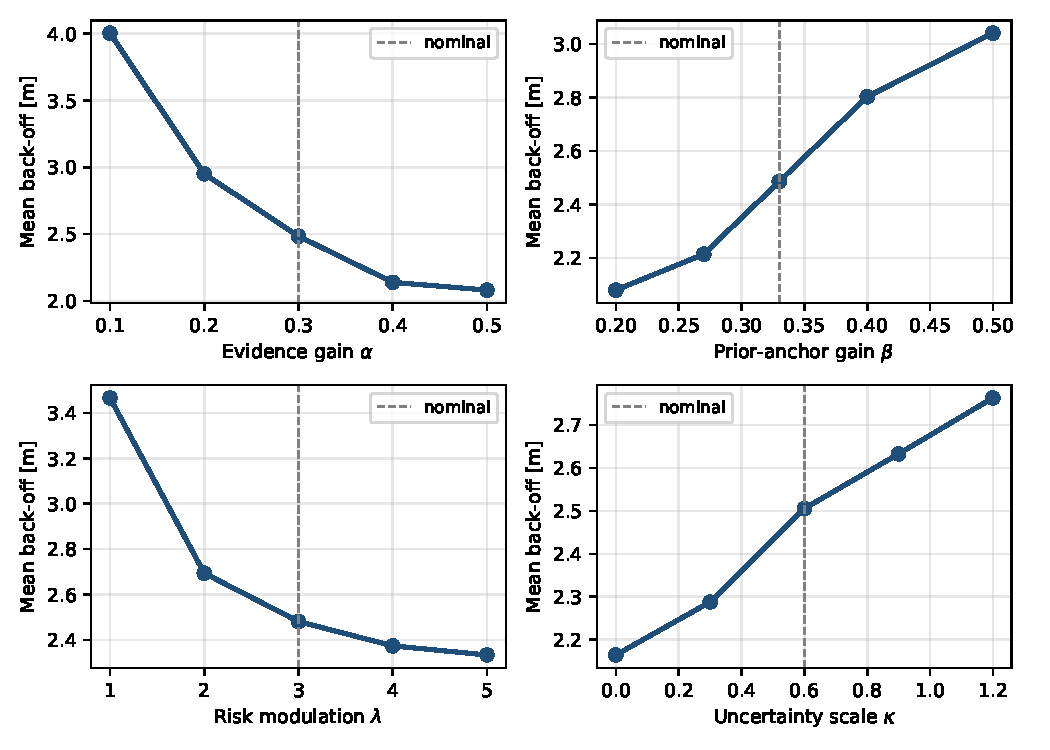
\includegraphics[width=\linewidth]{fig_sensitivity.pdf}
\caption{Parameter sensitivity on Scenario~A (adaptive controller).
Each panel varies one parameter while holding the others at nominal values.
Dashed vertical lines mark the nominal setting used in all experiments.
Mean back-off varies smoothly and remains below the fixed-$\delta=0.05$
baseline ($4.36$\,m, horizontal reference) across a wide neighborhood of
each parameter, indicating the closed-loop behavior is not tuned to a
knife-edge setting.}
\label{fig:sensitivity}
\end{figure}

Across all four sweeps, mean back-off changes gradually rather than
discontinuously, and the nominal operating point lies in the interior of a
flat region rather than at a corner.
The evidence gain~$\alpha$ has the largest effect: higher~$\alpha$ makes
the filter respond faster to prediction errors, raising back-off during
transients but also recovering faster afterward.
The prior-anchor gain~$\beta$ trades off the same erosion--recovery asymmetry
from the opposite direction.
Risk-modulation parameters~$\lambda$ and~$\kappa$ affect back-off magnitude
monotonically (higher~$\lambda$ or lower~$\kappa$ $\Rightarrow$ less
conservative at equal~$c$), consistent with Theorems~\ref{thm:feasible}
and~\ref{thm:cc}.
No parameter value in the tested ranges produced a safety violation on the
representative Scenario~A trajectory, though the severe-regime Monte Carlo
study (Table~\ref{tab:montecarlo}, right column) remains the authoritative
stress test for calibration at the distribution level.


% =============================================================================
% LOCATION 3 — Refresh Table III numbers (optional, after 100-trial run)
% =============================================================================
% REPLACE your existing Table III with the contents of outputs/tab_montecarlo.tex
% OR paste directly:
% =============================================================================

% \begin{table}[t]
\centering
\caption{Monte Carlo results, $100$ trials per cell.}
\label{tab:montecarlo}
\small
\begin{tabular}{lcccc}
\toprule
 & \multicolumn{2}{c}{Moderate severity} & \multicolumn{2}{c}{Severe (stress test)} \\
Method & B.o.\ [m] & Viol.\ & B.o.\ [m] & Viol.\ \\
\midrule
Fixed $\delta=0.05$ & $4.36\pm0.00$ & $0\%$ & $4.36\pm0.00$ & $20\%$ \\
Worst-case fixed & $9.95\pm0.00$ & $0\%$ & $9.95\pm0.00$ & $10\%$ \\
Naive reactive & $2.45\pm0.24$ & $0\%$ & $2.57\pm0.33$ & $30\%$ \\
Confidence-adaptive & $2.57\pm0.14$ & $0\%$ & $2.62\pm0.16$ & $20\%$ \\
\bottomrule
\end{tabular}
\end{table}

% After a full 100-trial run:
%   MPLCONFIGDIR=.mplcache python run_all.py --mc-trials 100
% copy updated tab_montecarlo.tex into your paper and recompile.


% =============================================================================
% LOCATION 4 — Figure file paths in preamble (if figures live in a subfolder)
% =============================================================================
% Add to your main .tex preamble if figures are in ./figures/ :
%
%   \graphicspath{{./figures/}{./outputs/}}
%
% Then copy all PDFs from outputs/ into figures/:
%   cp outputs/fig_*.pdf figures/
% =============================================================================


% =============================================================================
% LOCATION 5 — Cross-reference checklist (search your main .tex and verify)
% =============================================================================
%  Figure                          Label
%  -----------------------------------------------
%  Fig 1  fig_confidence.pdf       fig:confidence   (existing)
%  Fig 2  fig_backoff.pdf          fig:backoff      (existing)
%  Fig 3  fig_traj.pdf             fig:traj         (existing)
%  Fig 4  fig_pedestrian.pdf       fig:pedestrian   (existing)
%  Fig 5  fig_intersection.pdf     fig:intersection (existing)
%  Fig 6  fig_montecarlo_combined  fig:montecarlo   (existing)
%  Fig 7  fig_sensitivity.pdf      fig:sensitivity  (NEW — add ref in Sec V-F)
%  Table I                        tab:allocation   (existing, Scenario C)
%  Table II                       tab:results      (existing, Scenarios A-B)
%  Table III                      tab:montecarlo   (existing, refresh numbers)
%  Table IV                       tab:runtime      (NEW — add ref in Sec V-E)
% =============================================================================


% =============================================================================
% LOCATION 6 — One-sentence additions to Conclusion (optional)
% =============================================================================
% Append to the experimental sentence in Section VI:
%
% ``Monte Carlo evaluation over $100$ randomized trials confirmed a
% $41\%$ mean back-off reduction with zero violations in the moderate
% regime (Table~\ref{tab:montecarlo}), solver runtimes below
% $4$\,ms on average (Table~\ref{tab:runtime}), and smooth parameter
% sensitivity around the nominal design (Fig.~\ref{fig:sensitivity}).''
% =============================================================================

%            (only if you remove duplicate Table III / Fig 6 from the snippet)
%
%  FIGURE FILES (copy from outputs/ into your paper figures folder)
%  --------
%  fig_confidence.pdf          -> Fig 1  (already in paper)
%  fig_backoff.pdf             -> Fig 2
%  fig_traj.pdf                -> Fig 3
%  fig_pedestrian.pdf          -> Fig 4
%  fig_intersection.pdf        -> Fig 5
%  fig_montecarlo_combined.pdf -> Fig 6
%  fig_sensitivity.pdf         -> Fig 7  (NEW)
%
%  TABLE FILES
%  -----------
%  tab_montecarlo.tex  -> replace existing Table III (label: tab:montecarlo)
%  tab_runtime.tex     -> NEW Table IV      (label: tab:runtime)
% ============================================================================


% =============================================================================
% LOCATION 1 — Section V-E (Monte Carlo Statistical Evaluation and Solver Runtime)
% =============================================================================
% FIND in your main .tex the subsection:
%   \subsection{Monte Carlo Statistical Evaluation and Solver Runtime}
%   \label{sec:montecarlo}
%
% AFTER Figure~\ref{fig:montecarlo} (Fig. 6) and AFTER Table~\ref{tab:montecarlo}
% (Table III), INSERT the following two blocks:
%   (1) Table IV — solver runtime          [NEW]
%   (2) Revised closing paragraph        [optional update]
% =============================================================================

% --- INSERT AFTER TABLE III (tab:montecarlo) -----------------------------

\begin{table}[t]
\centering
\caption{QP solver runtime over all Monte Carlo solves ($T_s=200$\,ms control period).}
\label{tab:runtime}
\small
\begin{tabular}{lcccc}
\toprule
Method & Mean [ms] & Median [ms] & 95th [ms] & Max [ms] \\
\midrule
Fixed & 3.8 & 3.8 & 4.2 & 38.4 \\
Worst-case & 4.2 & 3.9 & 5.4 & 111.2 \\
Naive & 3.9 & 3.8 & 4.9 & 32.8 \\
Adaptive & 3.8 & 3.8 & 4.0 & 25.7 \\
\bottomrule
\end{tabular}
\end{table}
% If you copied tab_runtime.tex next to main.tex, use instead:
% \begin{table}[t]
\centering
\caption{QP solver runtime over all Monte Carlo solves ($T_s=200$\,ms control period).}
\label{tab:runtime}
\small
\begin{tabular}{lcccc}
\toprule
Method & Mean [ms] & Median [ms] & 95th [ms] & Max [ms] \\
\midrule
Fixed & 3.8 & 3.8 & 4.2 & 38.4 \\
Worst-case & 4.2 & 3.9 & 5.4 & 111.2 \\
Naive & 3.9 & 3.8 & 4.9 & 32.8 \\
Adaptive & 3.8 & 3.8 & 4.0 & 25.7 \\
\bottomrule
\end{tabular}
\end{table}

% --- OPTIONAL: replace the "Solver runtime." paragraph in Section V-E with ---

Solver runtime.
Table~\ref{tab:runtime} reports wall-clock QP solve time pooled over all
Monte Carlo solves (${\approx}40{,}000$ QPs across both severity regimes and
four methods, general-purpose CPU).
Mean solve time is \textbf{3.8\,ms} (median 3.8\,ms, 95th percentile
4.0\,ms), comfortably inside the $T_s=200$\,ms control period used throughout.
The confidence update (Proposition~1) is a closed-form scalar computation and
contributes negligible overhead relative to the QP solve.
A small tail of solves (maximum 111\,ms on worst-case runs) corresponds to
OSQP returning an inaccurate solution and triggering the SCS fallback; a
deployed system would use a solve-time watchdog (reuse previous input or
emergency maneuver), which we flag as implementation detail rather than a
theoretical limitation.


% =============================================================================
% LOCATION 2 — NEW subsection AFTER Section V-E, BEFORE Section VI (Conclusion)
% =============================================================================
% FIND in your main .tex:
%   \section{Conclusion}
%
% INSERT the entire block below IMMEDIATELY BEFORE \section{Conclusion}
% =============================================================================

\subsection{Parameter Sensitivity Analysis}
\label{sec:sensitivity}

Section~V introduced four tuning parameters with distinct roles:
$\alpha$ and~$\beta$ govern the MAP confidence filter (Proposition~1),
$\lambda$ modulates how quickly admissible risk $\delta(c)$ grows with
confidence (Eq.~\eqref{eq:delta-of-c}), and~$\kappa$ scales the effective
uncertainty $\sigma_{\mathrm{eff}}(c)$ (Eq.~\eqref{eq:sigma-eff}).
ACC reviewers reasonably ask whether performance is fragile to these choices;
Fig.~\ref{fig:sensitivity} answers this with a one-at-a-time sweep on
Scenario~A using the adaptive controller, holding all other parameters at
their nominal values ($\alpha=0.30$, $\beta=0.33$, $\lambda=3$, $\kappa=0.6$).

\begin{figure}[t]
\centering
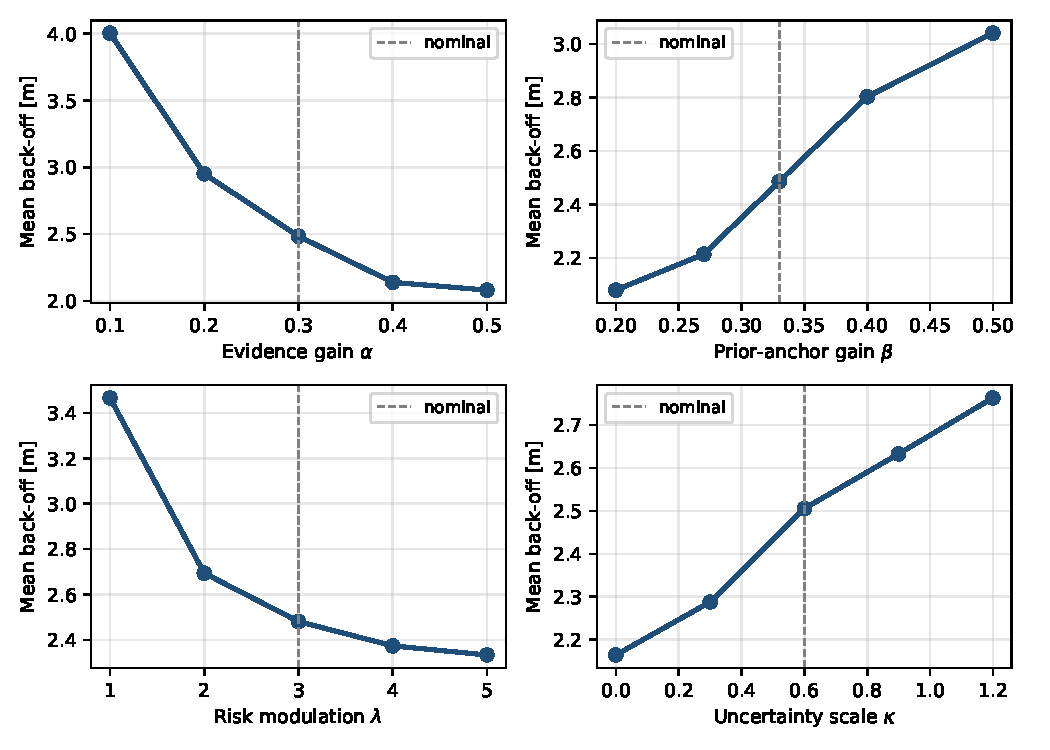
\includegraphics[width=\linewidth]{fig_sensitivity.pdf}
\caption{Parameter sensitivity on Scenario~A (adaptive controller).
Each panel varies one parameter while holding the others at nominal values.
Dashed vertical lines mark the nominal setting used in all experiments.
Mean back-off varies smoothly and remains below the fixed-$\delta=0.05$
baseline ($4.36$\,m, horizontal reference) across a wide neighborhood of
each parameter, indicating the closed-loop behavior is not tuned to a
knife-edge setting.}
\label{fig:sensitivity}
\end{figure}

Across all four sweeps, mean back-off changes gradually rather than
discontinuously, and the nominal operating point lies in the interior of a
flat region rather than at a corner.
The evidence gain~$\alpha$ has the largest effect: higher~$\alpha$ makes
the filter respond faster to prediction errors, raising back-off during
transients but also recovering faster afterward.
The prior-anchor gain~$\beta$ trades off the same erosion--recovery asymmetry
from the opposite direction.
Risk-modulation parameters~$\lambda$ and~$\kappa$ affect back-off magnitude
monotonically (higher~$\lambda$ or lower~$\kappa$ $\Rightarrow$ less
conservative at equal~$c$), consistent with Theorems~\ref{thm:feasible}
and~\ref{thm:cc}.
No parameter value in the tested ranges produced a safety violation on the
representative Scenario~A trajectory, though the severe-regime Monte Carlo
study (Table~\ref{tab:montecarlo}, right column) remains the authoritative
stress test for calibration at the distribution level.


% =============================================================================
% LOCATION 3 — Refresh Table III numbers (optional, after 100-trial run)
% =============================================================================
% REPLACE your existing Table III with the contents of outputs/tab_montecarlo.tex
% OR paste directly:
% =============================================================================

% \begin{table}[t]
\centering
\caption{Monte Carlo results, $100$ trials per cell.}
\label{tab:montecarlo}
\small
\begin{tabular}{lcccc}
\toprule
 & \multicolumn{2}{c}{Moderate severity} & \multicolumn{2}{c}{Severe (stress test)} \\
Method & B.o.\ [m] & Viol.\ & B.o.\ [m] & Viol.\ \\
\midrule
Fixed $\delta=0.05$ & $4.36\pm0.00$ & $0\%$ & $4.36\pm0.00$ & $20\%$ \\
Worst-case fixed & $9.95\pm0.00$ & $0\%$ & $9.95\pm0.00$ & $10\%$ \\
Naive reactive & $2.45\pm0.24$ & $0\%$ & $2.57\pm0.33$ & $30\%$ \\
Confidence-adaptive & $2.57\pm0.14$ & $0\%$ & $2.62\pm0.16$ & $20\%$ \\
\bottomrule
\end{tabular}
\end{table}

% After a full 100-trial run:
%   MPLCONFIGDIR=.mplcache python run_all.py --mc-trials 100
% copy updated tab_montecarlo.tex into your paper and recompile.


% =============================================================================
% LOCATION 4 — Figure file paths in preamble (if figures live in a subfolder)
% =============================================================================
% Add to your main .tex preamble if figures are in ./figures/ :
%
%   \graphicspath{{./figures/}{./outputs/}}
%
% Then copy all PDFs from outputs/ into figures/:
%   cp outputs/fig_*.pdf figures/
% =============================================================================


% =============================================================================
% LOCATION 5 — Cross-reference checklist (search your main .tex and verify)
% =============================================================================
%  Figure                          Label
%  -----------------------------------------------
%  Fig 1  fig_confidence.pdf       fig:confidence   (existing)
%  Fig 2  fig_backoff.pdf          fig:backoff      (existing)
%  Fig 3  fig_traj.pdf             fig:traj         (existing)
%  Fig 4  fig_pedestrian.pdf       fig:pedestrian   (existing)
%  Fig 5  fig_intersection.pdf     fig:intersection (existing)
%  Fig 6  fig_montecarlo_combined  fig:montecarlo   (existing)
%  Fig 7  fig_sensitivity.pdf      fig:sensitivity  (NEW — add ref in Sec V-F)
%  Table I                        tab:allocation   (existing, Scenario C)
%  Table II                       tab:results      (existing, Scenarios A-B)
%  Table III                      tab:montecarlo   (existing, refresh numbers)
%  Table IV                       tab:runtime      (NEW — add ref in Sec V-E)
% =============================================================================


% =============================================================================
% LOCATION 6 — One-sentence additions to Conclusion (optional)
% =============================================================================
% Append to the experimental sentence in Section VI:
%
% ``Monte Carlo evaluation over $100$ randomized trials confirmed a
% $41\%$ mean back-off reduction with zero violations in the moderate
% regime (Table~\ref{tab:montecarlo}), solver runtimes below
% $4$\,ms on average (Table~\ref{tab:runtime}), and smooth parameter
% sensitivity around the nominal design (Fig.~\ref{fig:sensitivity}).''
% =============================================================================
